\documentclass[a4paper,11pt,openright]{report}
\setlength{\parindent}{0pt} % set noindent for entire file

\usepackage[utf8]{inputenc}
\usepackage[a4paper,top=20mm,bottom=25mm,left=10mm,right=10mm]{geometry}
\usepackage{xcolor,graphicx}
\usepackage{amsmath}
\usepackage{setspace}
\usepackage{sectsty}
\usepackage{etoolbox}
\usepackage{enumitem}
\usepackage{listings}
\usepackage{times}

\graphicspath{ {/home/saran/Analytics/May_05/} }

\lstdefinestyle{mystyle}{
	backgroundcolor=\color{white},
	basicstyle=\ttfamily\footnotesize,
	breakatwhitespace=false,
	breaklines=true,
	captionpos=b,
	keepspaces=true,
	showspaces=false,
	showstringspaces=false,
	showtabs=false,
	tabsize=4
}

\lstset{style=mystyle}

\begin{document}
\singlespacing
\pagestyle{plain}

\begin{center}
\textbf{Assignment T-test} \\
Date: 05/05/2020 \hspace{2mm} Name: D.Saravanan
\end{center}

\vspace{10px}

T-test test the null hypothesis $H_{0}$ against the alternative hypothesis $H_{1}$. \\

For univariate samples, T-test performs a Student $t$ test. The test statistic is assumed to
follow a Student T-Distribution $[df]$. \\ 

For multivariate samples, T-test performs Hotelling's $T^{2}$ test. The test statistic is
assumed to follow a Hotelling T-Square Distribution $[p,df]$ where $p$ is the dimension of
data. \\

The degrees of freedom df, used to specify the distribution of the test statistic, depend on
the sample size, number of samples, and in the case of two univariate samples, the results 
of a test for equal variances. \\ 

For the T-test, a cutoff $\alpha$ is chosen such that $H_{0}$ is rejected only if $p < 
\alpha$. The value of $\alpha$ used for the "Test Conclusion" and "Short Test Conclusion"
properties is controlled by the Significance Level option. This value $\alpha$ is also used
in diagnostic tests of assumptions, including tests for normality, equal variance, and
symmetry. By default, $\alpha$ is set to $0.05$. \\

\vspace{1cm}

\begin{enumerate}

\item[1.] Certain refined edible oil is packed in tins holding 16 kg each. The filling
machine can maintain this but with a standard deviation of 0.5 kg. Samples of 25 are taken
from the production line. If a sample means are (i) 16.35 kg, (ii) 15.8 kg. Can we be 95 per
cent sure that the sample has come from a population of 16 kg tins? \\

\textbf{Solution:}

\textbf{Null hypothesis:} $H_{0}: \mu = 16$ \\
\textbf{Alternative hypothesis:} $H_{1}: \mu \neq 16$ 

\begin{enumerate}
\item[(i)] $\bar x = 16.35$, $s = 0.5$ and $n = 25$ 

\begin{equation*}
t = \frac{\bar x - \mu}{s/\sqrt{n}}
  = \frac{16.35 - 16}{0.5/\sqrt{25}} 
  = 3.5
\end{equation*}

\item[(ii)] $\bar x = 15.8$, $s = 0.5$ and $n = 25$

\begin{equation*}
t = \frac{\bar x - \mu}{s/\sqrt{n}}
  = \frac{15.8 - 16}{0.5/\sqrt{25}}
  = -2.0
\end{equation*}	

\end{enumerate}

\vspace{1cm}

Program:
\lstinputlisting[language=Python]{tscript.py}

\vspace{1cm}

Output:
\lstinputlisting{toutput1a.txt}

%figure_1
\begin{figure}[ht!]
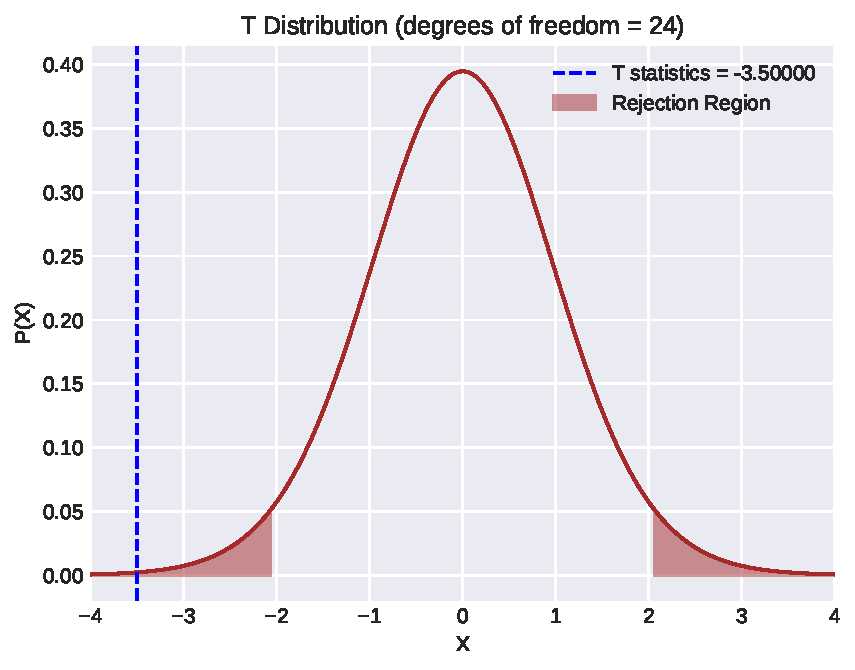
\includegraphics[width=16cm,height=8cm,keepaspectratio]{tscript1a.pdf}
\centering
\end{figure}

\vspace{2cm} 
\lstinputlisting{toutput1b.txt}

%figure_2
\begin{figure}[ht!]
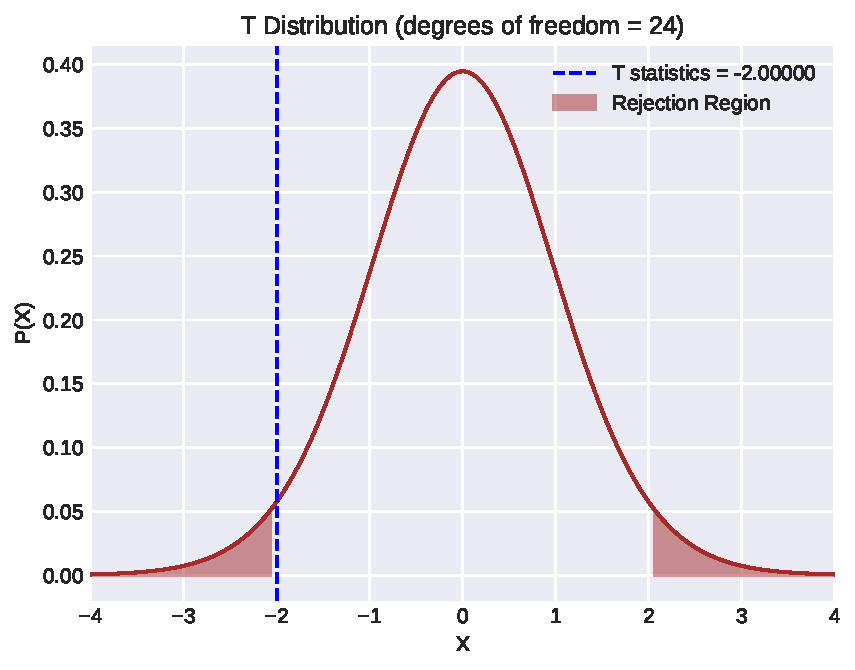
\includegraphics[width=16cm,height=8cm,keepaspectratio]{tscript1b.pdf}
\centering
\end{figure}

\item[2.] A filling machine is expected to fill 5 Kg of powder into bags. A sample of 10 
bags gave the weighs 4.7, 4.9, 5.0, 5.1, 5.4, 5.2, 4.6, 5.1, 4.6 and 4.7 Test whether the
machine is working properly. \\

Null hypothesis: $H_{0}: \mu = 5$ \\
Alternative hypothesis: $H_{1}: \mu \neq 5$ \\

Sample mean:
\begin{equation*}
\bar x =  \frac{\sum\limits_{i=1}^{n} x_{i}}{n} 
	= \frac{4.7 + 4.9 + 5.0 + 5.1 + 5.4 + 5.2 + 4.6 + 5.1 + 4.6 + 4.7}{10} 
	= 4.93
\end{equation*}

Sample variance:
\begin{equation*}
s^{2} = \frac{\sum\limits_{i=1}^{n} (x_{i} - \bar x)^{2}}{n - 1} 
	= \frac{\sum\limits_{i=1}^{10} (x_{i} - 4.93)^{2}}{10-1} 
	= 0.07567
\end{equation*}

Sample standard deviation:
\begin{equation*}
s = \sqrt{\frac{\sum\limits_{i=1}^{n} (x_{i} - \bar x)^{2}}{n - 1}}
= \sqrt{\frac{\sum\limits_{i=1}^{10} (x_{i} - 4.93)^{2}}{10 - 1}}
= \sqrt{0.07567} = 0.275076
\end{equation*}

T-statistics:
\begin{equation*}
t = \frac{\bar x - \mu}{s/\sqrt{n}} = \frac{4.93 - 5}{0.275076/\sqrt{10}} = -0.80472
\end{equation*}

Standard Error:
\begin{equation*}
S.E = \frac{s}{\sqrt{n}} = \frac{0.275076}{\sqrt{10}} = 0.08699
\end{equation*}

\vspace{2cm}

Program:
\lstinputlisting[language=Python]{tscript2.py}

\vspace{1cm}

Output:
\lstinputlisting{toutput2.txt}

%figure_3
\begin{figure}[ht!]
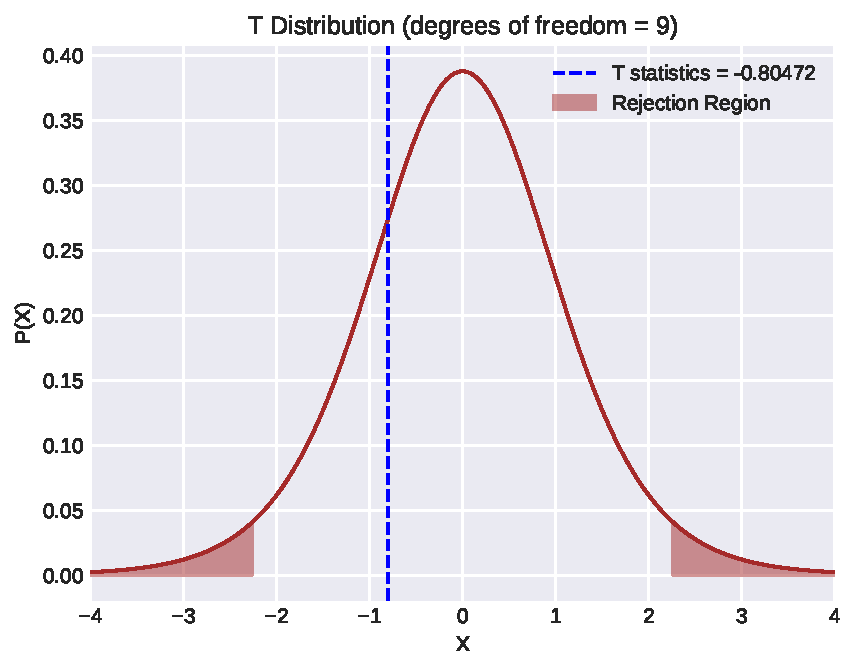
\includegraphics[width=16cm,height=8cm,keepaspectratio]{tscript2.pdf}
\centering
\end{figure}

\pagebreak

\vspace{2cm}

\item[3.] Two sets of ten students selected at random from a college were taken. One set was
given memory test as they were and the other was given the memory test after two weeks of
training and the scores are given below. \\
\begin{tabular}{lrrrrrrrrrr}
Set A: & 10 & 8 & 7 & 9 & 8 & 10 & 9 & 6 & 7 & 8 \\
Set B: & 12 & 8 & 8 & 10 & 8 & 11 & 9 & 8 & 9 & 9 \\
\end{tabular} \\
Do you think there is a significant effect due to training? \\

Null hypothesis: $H_{0}: \mu 1 = \mu 2$ \\
Alternative hypothesis: $H_{1}: \mu 1 \neq \mu 2$ \\

Set A: \\ 
\hspace*{10mm} Mean:
\begin{equation*}
\bar x_{1} = \frac{\sum\limits_{i=1}^{n1} x_{1i}}{n1}
    	= \frac{10 + 8 + 7 + 9 + 8 + 10 + 9 + 6 + 7 + 8}{10}
    	= 8.2
\end{equation*}

\hspace*{10mm} Variance:
\begin{equation*}
s_{1}^{2} = \frac{\sum\limits_{i=1}^{n1} (x_{1i} - \bar {x_{1}})^{2}}{n1 - 1}
		= \frac{\sum\limits_{i=1}^{10} (x_{1i} - 8.2)^{2}}{10 -1} = 1.73333
\end{equation*}

\hspace*{10mm} Standard Deviation:
\begin{equation*}
s_{1} = \sqrt{\frac{\sum\limits_{i=1}^{n1} (x_{1i} - \bar {x_{1}})^{2}}{n1 - 1}}
	= \sqrt{\frac{\sum\limits_{i=1}^{10} (x_{1i} - 8.2)^{2}}{10 -1}}
	= \sqrt{1.73333} = 1.31656
\end{equation*}

Set B: \\
\hspace*{10mm} Mean:
\begin{equation*}
\bar x_{2} = \frac{\sum\limits_{i=1}^{n2} x_{2i}}{n2}
	= \frac{12 + 8 + 8 + 10 + 8 + 11 + 9 + 8 + 9 + 9}{10}
	= 9.2
\end{equation*}

\hspace*{10mm} Variance:
\begin{equation*}
s_{2}^{2} = \frac{\sum\limits_{i=1}^{n2} (x_{2i} - \bar {x_{2}})^{2}}{n2 - 1}
= \frac{\sum\limits_{i=1}^{10} (x_{2i} - 9.2)^{2}}{10 -1} = 1.95556
\end{equation*}

\hspace*{10mm} Standard Deviation:
\begin{equation*}
s_{2} = \sqrt{\frac{\sum\limits_{i=1}^{n2} (x_{2i} - \bar x_{2})^{2}}{n2 - 1}}
= \sqrt{\frac{\sum\limits_{i=1}^{10} (x_{2i} - 9.2)^{2}}{10 -1}}
= \sqrt{1.95556} = 1.39841
\end{equation*}

Calculation of $s1/s2$:
\begin{equation*}
\frac{s_{1}}{s_{2}} = \frac{1.31656}{1.39841} = 0.94147
\end{equation*}

Test statistic: 
\begin{equation*}
		T = \frac{\bar x_{1} - \bar x_{2}}{\sqrt{s_{1}^{2}/n1 + s_{2}^{2}/n2}}
\end{equation*}

where $n1$ and $n2$ are the sample sizes, $\bar x_{1}$ and $\bar x_{2}$ are the sample
means, and $s_{1}^{2}$ and $s_{2}^{2}$ are the sample variances. 

If equal variances are assumed $(0.5 < s1/s2 < 2)$, then the formula reduces to:
\begin{equation*}
T = \frac{\bar x_{1} - \bar x_{2}}{s_{p} \sqrt{1/n1 + 1/n2}}
\end{equation*}

where
\begin{equation*}
s_{p}^{2} = \frac{(n1-1)s_{1}^{2} + (n2-1)s_{2}^{2}}{n1+n2-2}
\end{equation*}

Calculation of $s_{p}$:
\begin{equation*}
s_{p} = \sqrt{\frac{(10-1) \times 1.31656^{2} + (10-1) \times 1.39841^{2}}{10+10-2}} 
      = 1.35810
\end{equation*}

Calculation of T statistic:
\begin{equation*}
T = \frac{8.2 - 9.2}{1.35810 \times \sqrt{1/10 + 1/10}} = -1.64646
\end{equation*}

Calculation of Standard Error:
\begin{equation*}
S.E = sp \sqrt{1/n1 + 1/n2} = 1.35810 \times \sqrt{1/10 + 1/10} = 0.60736
\end{equation*}

\vspace{3cm}

Program:
\lstinputlisting[language=Python]{tscript3.py}

\vspace{2cm}

Output:
\lstinputlisting{toutput31.txt}

%figure_4
\begin{figure}[ht!]
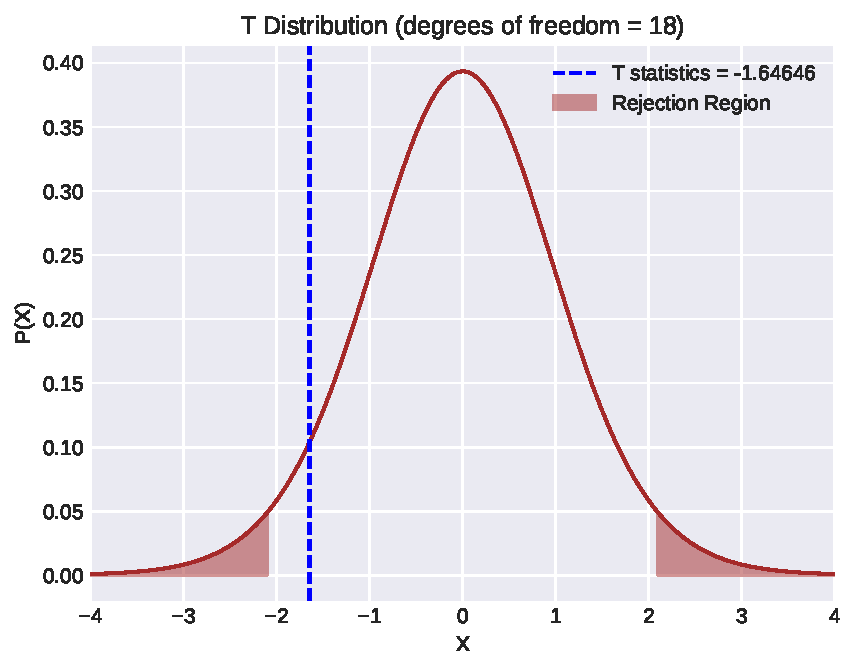
\includegraphics[width=16cm,height=8cm,keepaspectratio]{tscript3.pdf}
\centering
\end{figure}

\pagebreak

\vspace{3cm}

Program: T-test with in-built scipy.stats.ttest
\lstinputlisting[language=Python]{ttest2.py}

\vspace{2cm}

Output:
\lstinputlisting{toutput32.txt}

%figure_4
\begin{figure}[ht!]
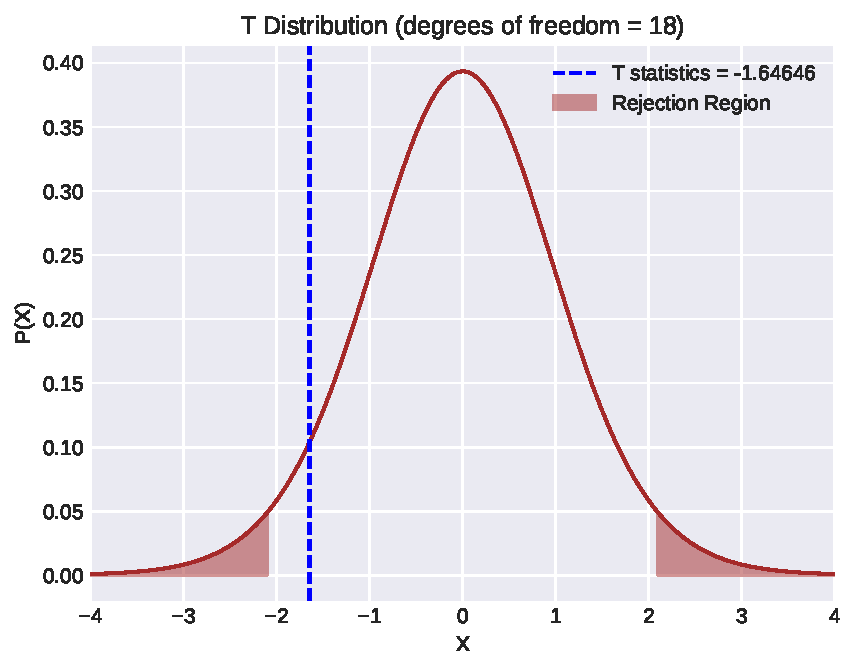
\includegraphics[width=16cm,height=8cm,keepaspectratio]{ttest2.pdf}
\centering
\end{figure}

\end{enumerate}
\end{document}
